% historybuttons-annote.ajr
% Created by FlowframTk version 0.8.5
% 3 May 2024, 14:18:30
\iffalse
% This image may require the following commands in the preamble:
\usepackage{ifpdf}
\makeatletter
\newcommand*{\jdroutline}[3]{%
  \GenericWarning{}{text outline can't be implemented}#3%
}%
\ifpdf
 \let\jdrorgmod\mod
 \InputIfFileExists{pdf-trans}%
 {%
   \renewcommand*{\jdroutline}[3]{%
     {\def\mod{\expandtwonumexprafter \modulo}%
     \setbox\@tempboxa\hbox{##3}%
     \boxgs{##1}{}\copy\@tempboxa
     }%
   }%
 }{}
 \let\mod\jdrorgmod
\else
 \IfFileExists{pst-char.sty}%
 {%
   \usepackage{pst-char}
   \renewcommand*{\jdroutline}[3]{%
     \begin{pspicture}(0,0)
     \pscharpath[##2]{##3}
     \end{pspicture}
   }
 }{}
\fi
\makeatother
\usepackage{pgf}
\usepgflibrary{decorations.text}
% The normal size font is assumed to be 10pt
% End of preamble information
\fi
\begin{pgfpicture}
\pgfpathmoveto{\pgfpoint{100.0bp}{827.890625bp}}
\pgfpathlineto{\pgfpoint{232.0bp}{979.46875bp}}
\pgfusepath{use as bounding box}
\begin{pgfscope}
\pgftransformcm{1.0}{0.0}{0.0}{1.0}{\pgfpoint{100.0bp}{931.0bp}}
\pgflowlevelsynccm
\pgfputat{\pgfpoint{0pt}{0pt}}{\pgftext[top,left]{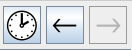
\includegraphics[width=132.0bp,height=50.0bp]{historybuttons}}}
\end{pgfscope}
\begin{pgfscope}
\pgfsetlinewidth{1.0bp}
\pgfsetrectcap
\pgfsetmiterjoin
\pgfsetmiterlimit{10.0}
\pgfpathmoveto{\pgfpoint{120.0bp}{961.0bp}}
\pgfpathlineto{\pgfpoint{120.0bp}{931.0bp}}
\definecolor{strokepaint}{rgb}{0.0,0.0,0.0}\pgfsetstrokecolor{strokepaint}
\pgfusepath{stroke}
\end{pgfscope}
% marker type 7
{\begin{pgfscope}
\definecolor{fillpaint}{rgb}{0.0,0.0,0.0}\pgfsetfillcolor{fillpaint}
\pgfpathqmoveto{120.0bp}{929.0bp}
\pgfpathqlineto{116.0bp}{937.0bp}
\pgfpathqlineto{120.0bp}{934.0bp}
\pgfpathqlineto{124.0bp}{937.0bp}
\pgfclosepath
\pgfusepathqfill
\end{pgfscope}}
\begin{pgfscope}
\pgftransformcm{1.0}{0.0}{0.0}{1.0}{\pgfpoint{110.0bp}{971.0bp}}
\pgftext[left,base]{\rmfamily\mdseries\upshape\large\color[rgb]{0.0,0.0,0.0}open history frame}
\end{pgfscope}
\begin{pgfscope}
\pgfsetlinewidth{1.0bp}
\pgfsetrectcap
\pgfsetmiterjoin
\pgfsetmiterlimit{10.0}
\pgfpathmoveto{\pgfpoint{140.0bp}{861.0bp}}
\pgfpathlineto{\pgfpoint{160.0bp}{881.0bp}}
\definecolor{strokepaint}{rgb}{0.0,0.0,0.0}\pgfsetstrokecolor{strokepaint}
\pgfusepath{stroke}
\end{pgfscope}
% marker type 7
{\begin{pgfscope}
\definecolor{fillpaint}{rgb}{0.0,0.0,0.0}\pgfsetfillcolor{fillpaint}
\pgfpathqmoveto{161.414215bp}{882.414215bp}
\pgfpathqlineto{158.585785bp}{873.928925bp}
\pgfpathqlineto{157.878677bp}{878.878677bp}
\pgfpathqlineto{152.928925bp}{879.585785bp}
\pgfclosepath
\pgfusepathqfill
\end{pgfscope}}
\begin{pgfscope}
\pgftransformcm{1.0}{-0.0}{0.0}{1.0}{\pgfpoint{135.65625bp}{859.359375bp}}
\pgftext[right,top]{\rmfamily\mdseries\upshape\large\color[rgb]{0.0,0.0,0.0}back}
\end{pgfscope}
\begin{pgfscope}
\pgfsetlinewidth{1.0bp}
\pgfsetrectcap
\pgfsetmiterjoin
\pgfsetmiterlimit{10.0}
\pgfpathmoveto{\pgfpoint{210.0bp}{841.0bp}}
\pgfpathlineto{\pgfpoint{210.0bp}{881.0bp}}
\definecolor{strokepaint}{rgb}{0.0,0.0,0.0}\pgfsetstrokecolor{strokepaint}
\pgfusepath{stroke}
\end{pgfscope}
% marker type 7
{\begin{pgfscope}
\definecolor{fillpaint}{rgb}{0.0,0.0,0.0}\pgfsetfillcolor{fillpaint}
\pgfpathqmoveto{210.0bp}{883.0bp}
\pgfpathqlineto{214.0bp}{875.0bp}
\pgfpathqlineto{210.0bp}{878.0bp}
\pgfpathqlineto{206.0bp}{875.0bp}
\pgfclosepath
\pgfusepathqfill
\end{pgfscope}}
\begin{pgfscope}
\pgftransformcm{1.0}{-0.0}{0.0}{1.0}{\pgfpoint{211.78125bp}{836.46875bp}}
\pgftext[right,top]{\rmfamily\mdseries\upshape\large\color[rgb]{0.0,0.0,0.0}forwards}
\end{pgfscope}
\end{pgfpicture}
